\subsection{Настройка Apache Superset}\label{subsec:-apache-superset}
Это известное средство анализа и визуализации данных с открытым исходным кодом для настройки ``по кнопке``
требует ощутимого упорства.
Для автоматизации запуска Superset с предустановленными панелями потребовалась усиленная команда запуска ПО в виде:
\begin{itemize}
    \item Установки библиотек для подключения к целевой БД (PostgreSQL).
    \item Инициализации внутренней базы (которой по умолчанию является
    встроенная sqlite3, это решение хорошо подходит для демонстрации, но в продуктовой среде к использованию не
    рекомендуется).
    \item Инициализации самого Superset.
    \item Создания администратора с паролем.
    \item Ожидания запуска Superset по определённому порту.
    \item Запуска скрипта импорта с использованием API Superset, включающего:
    \begin{itemize}
        \item Получение токена для обращений по API\@.
        \item Импорту подготовленного архива с панелями и чартами.
    \end{itemize}
\end{itemize}

Существенной сложностью в отладке и построении данного процесса было диагностирование и обход требования
использования CSRF-токена для работы с flask-сервером, реализующим API Superset.
Изучались заголовки запросов в отладчике браузера, документация Superset, форумы и GPT-объяснения.
В результате в изначальные настройки программы, расположенные в python-скрипте были добавлены переменные,
отключающие механизм CSRF-токена и ослабляющие настройки безопасности на демонстрационном стенде.

\subsection{Панели}\label{subsec:supersetpanels}

Ниже приведена автоматически импортируемая панель.
График был собран из данных таблицы покупок, агрегированных по дате.
Чарт - из запроса по нескольким таблицам со связями.

\begin{figure}[htbp]
    \centering
    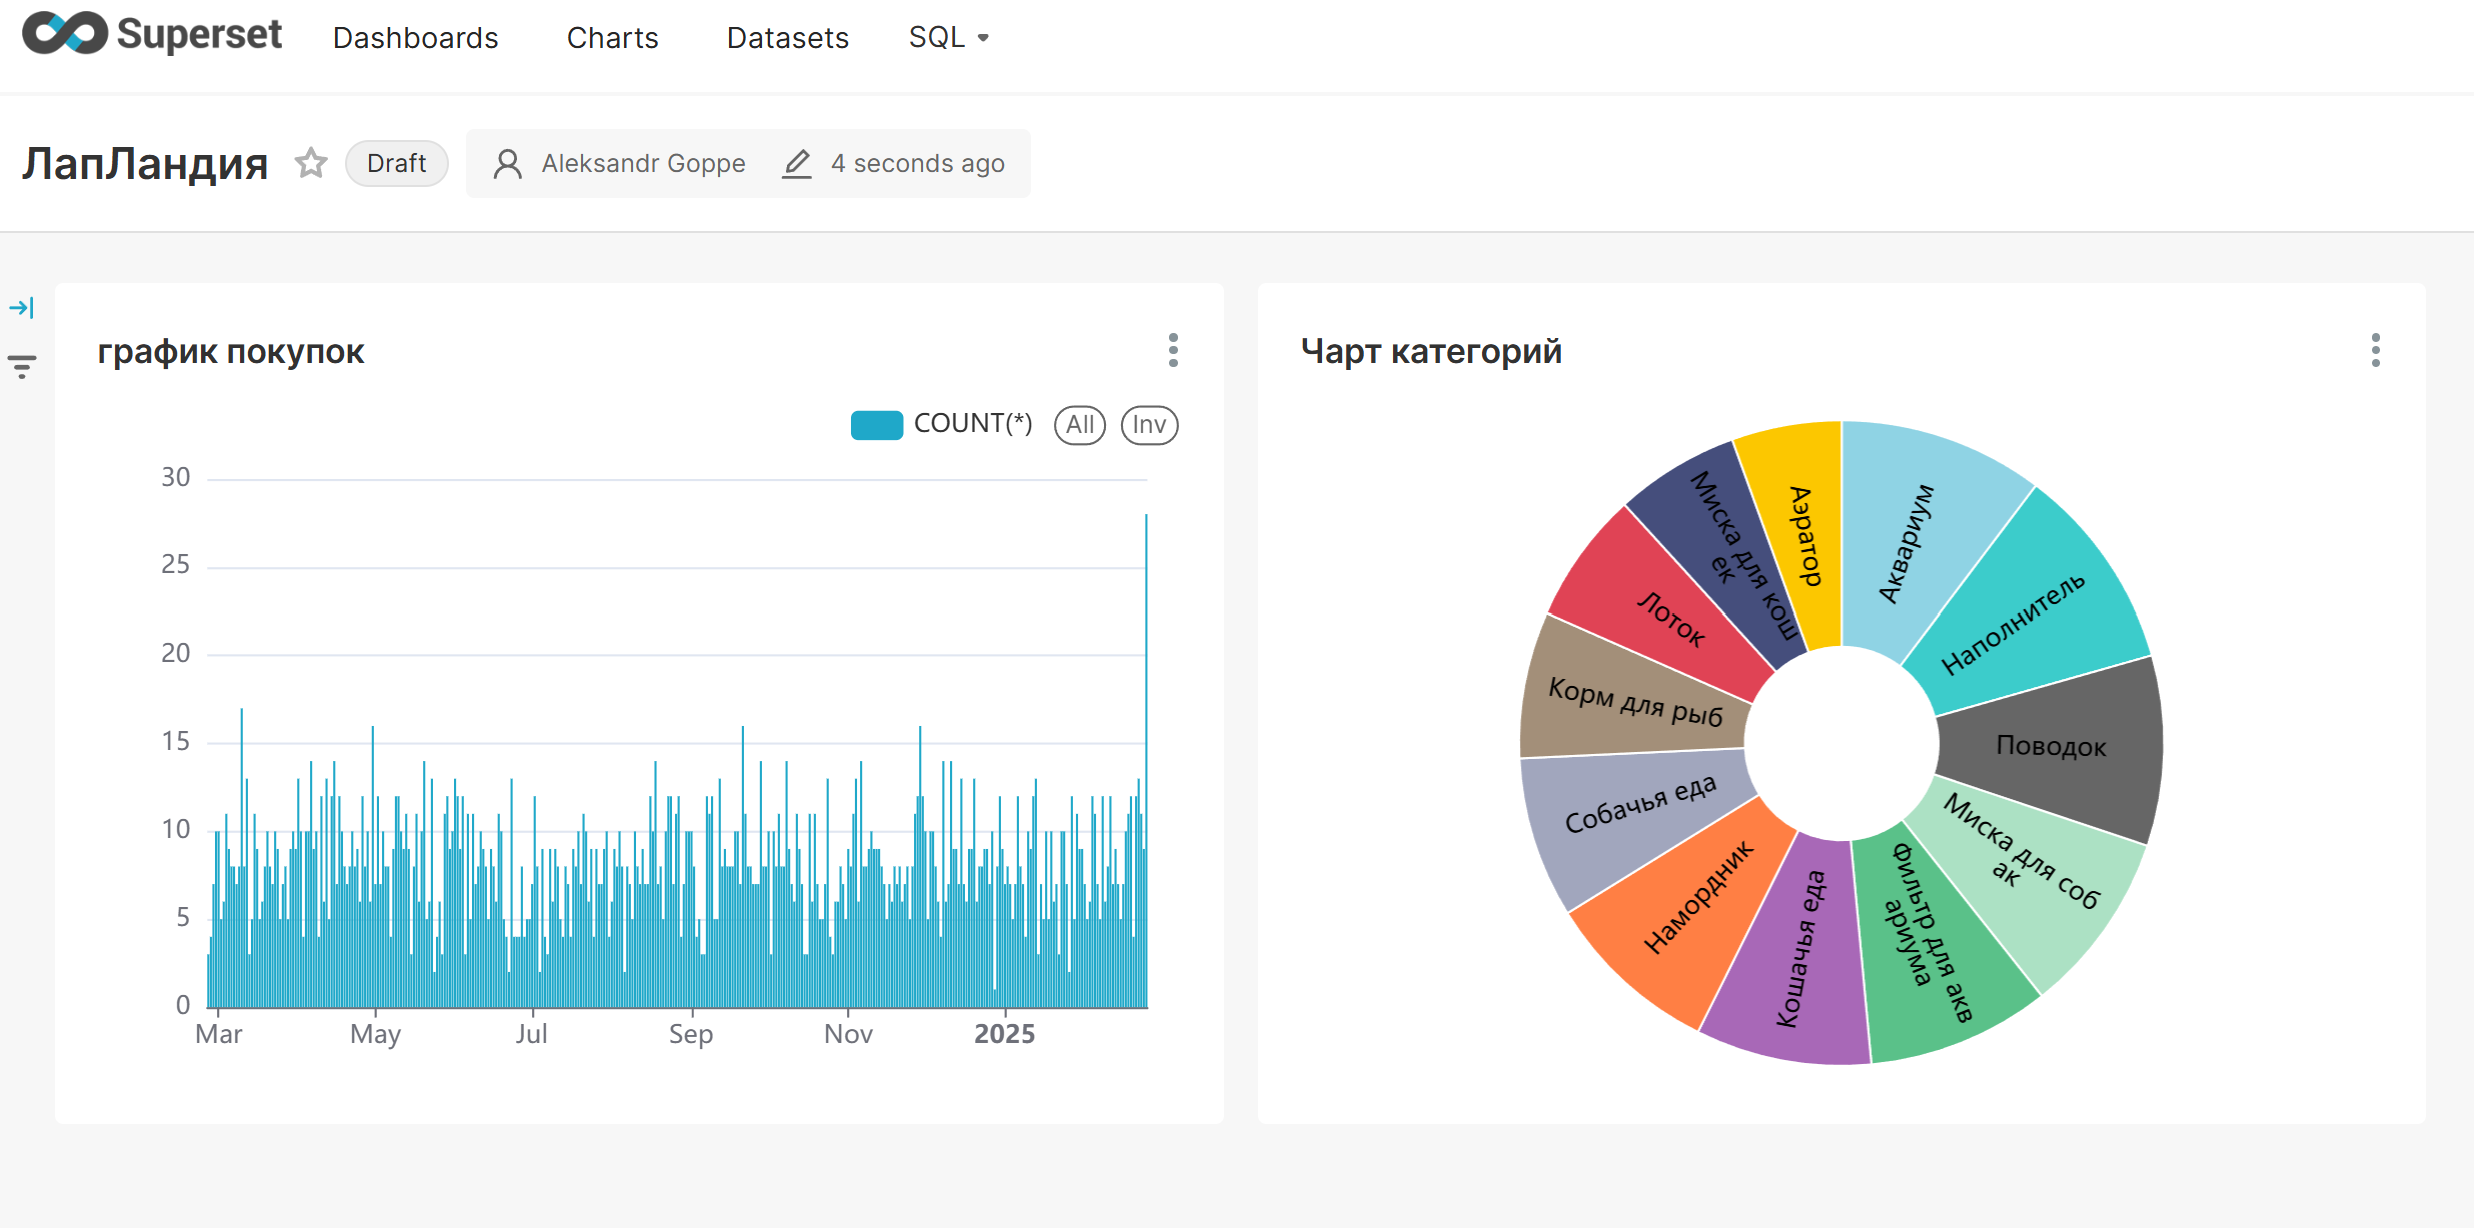
\includegraphics[width=0.9\textwidth]{superset} % Вставка изображения
    \caption{Панель в Superset}\label{fig:supersetpic}
\end{figure}